\documentclass[journal,12pt,twocolumn]{IEEEtran}

\usepackage{setspace}
\usepackage{gensymb}
\singlespacing
\usepackage[cmex10]{amsmath}

\usepackage{amsthm}

\usepackage{mathrsfs}
\usepackage{txfonts}
\usepackage{stfloats}
\usepackage{bm}
\usepackage{cite}
\usepackage{cases}
\usepackage{subfig}

\usepackage{longtable}
\usepackage{multirow}

\usepackage{enumitem}
\usepackage{mathtools}
\usepackage{steinmetz}
\usepackage{tikz}
\usepackage{circuitikz}
\usepackage{verbatim}
\usepackage{tfrupee}
\usepackage[breaklinks=true]{hyperref}
\usepackage{graphicx}
\usepackage{tkz-euclide}

\usetikzlibrary{calc,math}
\usepackage{listings}
    \usepackage{color}                                            %%
    \usepackage{array}                                            %%
    \usepackage{longtable}                                        %%
    \usepackage{calc}                                             %%
    \usepackage{multirow}                                         %%
    \usepackage{hhline}                                           %%
    \usepackage{ifthen}                                           %%
    \usepackage{lscape}     
\usepackage{multicol}
\usepackage{chngcntr}
\usepackage{hyperref}
\hypersetup{
    colorlinks=true,
    linkcolor=blue,
    filecolor=blue,      
    urlcolor=blue,
}
\DeclareMathOperator*{\Res}{Res}

\renewcommand\thesection{\arabic{section}}
\renewcommand\thesubsection{\thesection.\arabic{subsection}}
\renewcommand\thesubsubsection{\thesubsection.\arabic{subsubsection}}

\renewcommand\thesectiondis{\arabic{section}}
\renewcommand\thesubsectiondis{\thesectiondis.\arabic{subsection}}
\renewcommand\thesubsubsectiondis{\thesubsectiondis.\arabic{subsubsection}}


\hyphenation{op-tical net-works semi-conduc-tor}
\def\inputGnumericTable{}                                 %%

\lstset{
%language=C,
frame=single, 
breaklines=true,
columns=fullflexible
}

\makeatletter
\setlength{\@fptop}{0pt}
\makeatother

\begin{document}


\newtheorem{theorem}{Theorem}[section]
\newtheorem{problem}{Problem}
\newtheorem{proposition}{Proposition}[section]
\newtheorem{lemma}{Lemma}[section]
\newtheorem{corollary}[theorem]{Corollary}
\newtheorem{example}{Example}[section]
\newtheorem{definition}[problem]{Definition}

\newcommand{\BEQA}{\begin{eqnarray}}
\newcommand{\EEQA}{\end{eqnarray}}
\newcommand{\define}{\stackrel{\triangle}{=}}
\bibliographystyle{IEEEtran}
\raggedbottom
\setlength{\parindent}{0pt}
\providecommand{\mbf}{\mathbf}
\providecommand{\pr}[1]{\ensuremath{\Pr\left(#1\right)}}
\providecommand{\qfunc}[1]{\ensuremath{Q\left(#1\right)}}
\providecommand{\sbrak}[1]{\ensuremath{{}\left[#1\right]}}
\providecommand{\lsbrak}[1]{\ensuremath{{}\left[#1\right.}}
\providecommand{\rsbrak}[1]{\ensuremath{{}\left.#1\right]}}
\providecommand{\brak}[1]{\ensuremath{\left(#1\right)}}
\providecommand{\lbrak}[1]{\ensuremath{\left(#1\right.}}
\providecommand{\rbrak}[1]{\ensuremath{\left.#1\right)}}
\providecommand{\cbrak}[1]{\ensuremath{\left\{#1\right\}}}
\providecommand{\lcbrak}[1]{\ensuremath{\left\{#1\right.}}
\providecommand{\rcbrak}[1]{\ensuremath{\left.#1\right\}}}
\theoremstyle{remark}
\newtheorem{rem}{Remark}
\newcommand{\sgn}{\mathop{\mathrm{sgn}}}
\providecommand{\abs}[1]{$\left\vert#1\right\vert$}
\providecommand{\res}[1]{\Res\displaylimits_{#1}} 
\providecommand{\norm}[1]{$\left\lVert#1\right\rVert$}
%\providecommand{\norm}[1]{\lVert#1\rVert}
\providecommand{\mtx}[1]{\mathbf{#1}}
\providecommand{\mean}[1]{$E\left[ #1 \right]$}
\providecommand{\fourier}{\overset{\mathcal{F}}{ \rightleftharpoons}}
%\providecommand{\hilbert}{\overset{\mathcal{H}}{ \rightleftharpoons}}
\providecommand{\system}{\overset{\mathcal{H}}{ \longleftrightarrow}}
	%\newcommand{\solution}[2]{\textbf{Solution:}{#1}}
\newcommand{\solution}{\noindent \textbf{Solution: }}
\newcommand{\cosec}{\,\text{cosec}\,}
\providecommand{\dec}[2]{\ensuremath{\overset{#1}{\underset{#2}{\gtrless}}}}
\newcommand{\myvec}[1]{\ensuremath{\begin{pmatrix}#1\end{pmatrix}}}
\newcommand{\mydet}[1]{\ensuremath{\begin{vmatrix}#1\end{vmatrix}}}
\newcommand*{\permcomb}[4][0mu]{{{}^{#3}\mkern#1#2_{#4}}}
\newcommand*{\perm}[1][-3mu]{\permcomb[#1]{P}}
\newcommand*{\comb}[1][-1mu]{\permcomb[#1]{C}}
\numberwithin{equation}{subsection}
\makeatletter
\@addtoreset{figure}{problem}
\makeatother
\let\StandardTheFigure\thefigure
\let\vec\mathbf
\renewcommand{\thefigure}{\theproblem}
\def\putbox#1#2#3{\makebox[0in][l]{\makebox[#1][l]{}\raisebox{\baselineskip}[0in][0in]{\raisebox{#2}[0in][0in]{#3}}}}
     \def\rightbox#1{\makebox[0in][r]{#1}}
     \def\centbox#1{\makebox[0in]{#1}}
     \def\topbox#1{\raisebox{-\baselineskip}[0in][0in]{#1}}
     \def\midbox#1{\raisebox{-0.5\baselineskip}[0in][0in]{#1}}
\vspace{3cm}
\title{Assignment 3}
\author{Perambuduri Srikaran - AI20BTECH11018}
\maketitle
\newpage
\bigskip
\renewcommand{\thefigure}{\theenumi}
\renewcommand{\thetable}{\theenumi}
Download all python codes from
\begin{lstlisting}
https://github.com/srikaran-p/AI1103/tree/main/Assignment3/codes
\end{lstlisting}
and latex codes from 
\begin{lstlisting}
https://github.com/srikaran-p/AI1103/tree/main/Assignment3
\end{lstlisting}
\section*{Problem}
(GATE-MA 2015 Q17) Let $X$ be a random variable having the distribution function
\begin{align}
F(x) = 
    \begin{cases} 
      0 & \text{if }x < 0 \\
      \frac{1}{4} & \text{if } 0\leq x < 1 \\
      \frac{1}{3} & \text{if } 1\leq x < 2 \\
      \frac{1}{2} & \text{if } 2\leq x < \frac{11}{3} \\
      1 & \text{if } x \geq \frac{11}{3} \\
   \end{cases}
\end{align}
Then $E(X)$ is equal to ...
\section*{Solution}
Consider a unit step function $u(x)$,
\begin{align}
u(x) = 
    \begin{cases}
        1 & x \geq 0 \\
        0 & \text{otherwise}
    \end{cases}
\end{align}
We will remove the discontinuity at $x=0$ by defining $u_{\alpha}(x)$ for any $\alpha > 0$,
\begin{align}
u_{\alpha}(x) &= 
    \begin{cases}
        1 & x > \frac{\alpha}{2} \\
        \frac{1}{\alpha}(x + \frac{\alpha}{2}) & -\frac{\alpha}{2} \leq x \leq \frac{\alpha}{2} \\
        0 & x < -\frac{\alpha}{2}
    \end{cases}\\
\delta_{\alpha}(x) &= \frac{du_{\alpha}(x)}{dx}\\
\delta_{\alpha}(x) &=
    \begin{cases}
        \frac{1}{\alpha} & -\frac{\alpha}{2} \leq x \leq \frac{\alpha}{2} \\
        0 & |x| > \frac{\alpha}{2}
    \end{cases}\\
u(x) &= \lim_{\alpha \to 0} u_{\alpha}(x)\\
\delta (x) &= \lim_{\alpha \to 0} \delta_{\alpha}(x)
\end{align}
\begin{align}
    \int_{-\infty}^{\infty}g(x)\delta(x-x_0)dx = g(x_0) \label{eq:1}
\end{align}
We will add dirac $\delta$ functions to remove discontinuities in $F(x)$.
%We will add $\frac{1}{4}u(x) + \frac{1}{12}u(x - 1) + \frac{1}{6}u(x-2) + \frac{1}{2}u\brak{x-\frac{11}{3}}$ to $F(x)$
\begin{align}
    f_{X}(x) &= \frac{dF(x)}{dx}
\end{align}
\begin{multline}
    f_{X}(x) = \frac{1}{4}\delta(x) + \frac{1}{12}\delta(x - 1) + \frac{1}{6}\delta(x-2) +\\ \frac{1}{2}\delta\brak{x-\frac{11}{3}} + 0
\end{multline}
We will use \eqref{eq:1} to compute E(X)
\begin{align}
    E(X) = \int_{-\infty}^{\infty}xf_X(x)dx
\end{align}
\begin{multline}
    E(X) = \int_{-\infty}^{\infty}\frac{1}{4}x\delta(x) + \frac{1}{12}x\delta(x - 1) +\\ \frac{1}{6}x\delta(x-2) + \frac{1}{2}x\delta\brak{x-\frac{11}{3}}dx
\end{multline}
\begin{align}
    E(X) &= {\frac{1}{4}}\times 0 + {\frac{1}{12}}\times 1 + {\frac{1}{6}}\times 2 + {\frac{1}{2}}\times{\frac{11}{3}}\\
    E(X) &= 2.25
\end{align}
\section*{Alternative Solution}
\begin{align}
    E(g(X)) = \int_{-\infty}^{\infty} g(x)dF(x)
\end{align}
Suppose $F(x)$ is continuously differentiable on \sbrak{a,b} except at a finite number of points $c_1, c_2, \dots c_n$.\\
\begin{multline}
    \int_{a}^{b}g(x)dF(x) = \int_{a}^{c_1}g(x)dF(x) +\\ g(c_1)\sbrak{F(c_1) - \lim_{\substack{x \to c_1 \\ x < c_1}}F(x)} + \\ \int_{c_1}^{c_2}g(x)dF(x) + \\g(c_2)\sbrak{F(c_2) - \lim_{\substack{x \to c_2 \\ x < c_2}}F(x)} + \dots +\\ \int_{c_{n-1}}^{c_n}g(x)dF(x) +\\ g(c_n)\sbrak{F(c_n) - \lim_{\substack{x \to c_n \\ x < c_n}}F(x)} + \\ \int_{c_n}^{b}g(x)dF(x)
\end{multline}
As per the question, $g(X) = X$
\begin{align}
    E(X) = \int_{-\infty}^{\infty} xdF(x)
\end{align}
\begin{multline}
    E(X) = \int_{-\infty}^{0}xdF(x) + 0\sbrak{F(0) - \lim_{\substack{x \to 0 \\ x < 0}}F(x)} + \\ \int_{0}^{1}xdF(x) + 1\sbrak{F(1) - \lim_{\substack{x \to 1 \\ x < 1}}F(x)} + \\ \int_{1}^{2}xdF(x) + 2\sbrak{F(2) - \lim_{\substack{x \to 2 \\ x < 2}}F(x)} + \\ \int_{2}^{\frac{11}{3}}xdF(x) +  \frac{11}{3}\sbrak{F\brak{\frac{11}{3}} - \lim_{\substack{x \to \frac{11}{3} \\ x < \frac{11}{3}}}F(x)} +\\ \int_{\frac{11}{3}}^{\infty}xdF(x)
\end{multline}
\begin{multline}
    \int_{-\infty}^{0}xdF(x) = \int_{0}^{1}xdF(x) = \int_{1}^{2}xdF(x) = \\ \int_{2}^{\frac{11}{3}}xdF(x) = \int_{\frac{11}{3}}^{\infty}xdF(x) = 0
\end{multline}
\begin{align}
    E(X) = 2.25
\end{align}
\begin{figure}[hb]
    \centering
    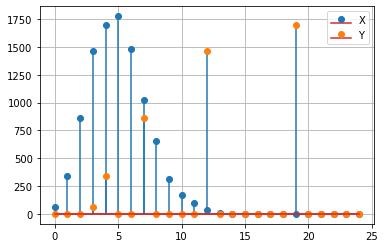
\includegraphics[width=\columnwidth]{Figure1.png}
    \caption{Plot for Simulation v/s Theoretical}
    \label{fig:plot}
\end{figure}
\end{document}